%% Beginning of file 'sample631.tex'
%%
%% Modified 2021 March
%%
%% This is a sample manuscript marked up using the
%% AASTeX v6.31 LaTeX 2e macros.
%%
%% AASTeX is now based on Alexey Vikhlinin's emulateapj.cls 
%% (Copyright 2000-2015).  See the classfile for details.

%% AASTeX requires revtex4-1.cls and other external packages such as
%% latexsym, graphicx, amssymb, longtable, and epsf.  Note that as of 
%% Oct 2020, APS now uses revtex4.2e for its journals but remember that 
%% AASTeX v6+ still uses v4.1. All of these external packages should 
%% already be present in the modern TeX distributions but not always.
%% For example, revtex4.1 seems to be missing in the linux version of
%% TexLive 2020. One should be able to get all packages from www.ctan.org.
%% In particular, revtex v4.1 can be found at 
%% https://www.ctan.org/pkg/revtex4-1.

%% The first piece of markup in an AASTeX v6.x document is the \documentclass
%% command. LaTeX will ignore any data that comes before this command. The 
%% documentclass can take an optional argument to modify the output style.
%% The command below calls the preprint style which will produce a tightly 
%% typeset, one-column, single-spaced document.  It is the default and thus
%% does not need to be explicitly stated.
%%
%% using aastex version 6.3
\documentclass[linenumbers,twocolumn]{aastex631}
%\documentclass[linenumbers]{aastex631}
%\documentclass[linenumbers,twocolumn]%{aastex631}
\usepackage[dvipsnames]{xcolor}
\usepackage{color}
\usepackage{makecell}
\usepackage{appendix}
\usepackage{mathrsfs}
\usepackage{longtable}
\usepackage{hyperref}
\hypersetup{colorlinks=true, urlcolor=blue}
%\usepackage[UTF8,heading = true]{ctex}
\frenchspacing
\newcommand{\ud}{\mathrm{d}}
\newcommand{\dirac}{\partial\llap{$\diagup$\kern-2pt}}
\newcommand{\fett}[1]{\boldsymbol{#1}}
\newcommand{\fettu}[1]{\mathbf{#1}}
\newcommand{\quabla}{\square}
\newcommand{\diag}{\mathrm{diag}}
\newcommand{\sgn}{\mathrm{sgn}}
\newcommand{\Tr}{\mathrm{Tr}}
\newcommand{\Heaviside}{\theta}
\newcommand{\eig}{\mathrm{eig}}
\newcommand{\e}{\mathrm{e}}
%% The default is a single spaced, 10 point font, single spaced article.
%% There are 5 other style options available via an optional argument. They
%% can be invoked like this:
%%
%% \documentclass[arguments]{aastex631}
%% 
%% where the layout options are:
%%
%%  twocolumn   : two text columns, 10 point font, single spaced article.
%%                This is the most compact and represent the final published
%%                derived PDF copy of the accepted manuscript from the publisher
%%  manuscript  : one text column, 12 point font, double spaced article.
%%  preprint    : one text column, 12 point font, single spaced article.  
%%  preprint2   : two text columns, 12 point font, single spaced article.
%%  modern      : a stylish, single text column, 12 point font, article with
%% 		  wider left and right margins. This uses the Daniel
%% 		  Foreman-Mackey and David Hogg design.
%%  RNAAS       : Supresses an abstract. Originally for RNAAS manuscripts 
%%                but now that abstracts are required this is obsolete for
%%                AAS Journals. Authors might need it for other reasons. DO NOT
%%                use \begin{abstract} and \end{abstract} with this style.
%%
%% Note that you can submit to the AAS Journals in any of these 6 styles.
%%
%% There are other optional arguments one can invoke to allow other stylistic
%% actions. The available options are:
%%
%%   astrosymb    : Loads Astrosymb font and define \astrocommands. 
%%   tighten      : Makes baselineskip slightly smaller, only works with 
%%                  the twocolumn substyle.
%%   times        : uses times font instead of the default
%%   linenumbers  : turn on lineno package.
%%   trackchanges : required to see the revision mark up and print its output
%%   longauthor   : Do not use the more compressed footnote style (default) for 
%%                  the author/collaboration/affiliations. Instead print all
%%                  affiliation information after each name. Creates a much 
%%                  longer author list but may be desirable for short 
%%                  author papers.
%% twocolappendix : make 2 column appendix.
%%   anonymous    : Do not show the authors, affiliations and acknowledgments 
%%                  for dual anonymous review.
%%
%% these can be used in any combination, e.g.
%%
%% \documentclass[twocolumn,linenumbers,trackchanges]{aastex631}
%%
%% AASTeX v6.* now includes \hyperref support. While we have built in specific
%% defaults into the classfile you can manually override them with the
%% \hypersetup command. For example,
%%
%% \hypersetup{linkcolor=red,citecolor=green,filecolor=cyan,urlcolor=magenta}
%%
%% will change the color of the internal links to red, the links to the
%% bibliography to green, the file links to cyan, and the external links to
%% magenta. Additional information on \hyperref options can be found here:
%% https://www.tug.org/applications/hyperref/manual.html#x1-40003
%%
%% Note that in v6.3 "bookmarks" has been changed to "true" in hyperref
%% to improve the accessibility of the compiled pdf file.
%%
%% If you want to create your own macros, you can do so
%% using \newcommand. Your macros should appear before
%% the \begin{document} command.
%%
\newcommand{\vdag}{(v)^\dagger}
\newcommand\aastex{AAS\TeX}
\newcommand\latex{La\TeX}
\usepackage{amsmath}

%% Reintroduced the \received and \accepted commands from AASTeX v5.2
%\received{March 1, 2021}
%\revised{April 1, 2021}
%\accepted{\today}

%% Command to document which AAS Journal the manuscript was submitted to.
%% Adds "Submitted to " the argument.
%\submitjournal{PSJ}

%% For manuscript that include authors in collaborations, AASTeX v6.31
%% builds on the \collaboration command to allow greater freedom to 
%% keep the traditional author+affiliation information but only show
%% subsets. The \collaboration command now must appear AFTER the group
%% of authors in the collaboration and it takes TWO arguments. The last
%% is still the collaboration identifier. The text given in this
%% argument is what will be shown in the manuscript. The first argument
%% is the number of author above the \collaboration command to show with
%% the collaboration text. If there are authors that are not part of any
%% collaboration the \nocollaboration command is used. This command takes
%% one argument which is also the number of authors above to show. A
%% dashed line is shown to indicate no collaboration. This example manuscript
%% shows how these commands work to display specific set of authors 
%% on the front page.
%%
%% For manuscript without any need to use \collaboration the 
%% \AuthorCollaborationLimit command from v6.2 can still be used to 
%% show a subset of authors.
%
%\AuthorCollaborationLimit=2
%
%% will only show Schwarz & Muench on the front page of the manuscript
%% (assuming the \collaboration and \nocollaboration commands are
%% commented out).
%%
%% Note that all of the author will be shown in the published article.
%% This feature is meant to be used prior to acceptance to make the
%% front end of a long author article more manageable. Please do not use
%% this functionality for manuscripts with less than 20 authors. Conversely,
%% please do use this when the number of authors exceeds 40.
%%
%% Use \allauthors at the manuscript end to show the full author list.
%% This command should only be used with \AuthorCollaborationLimit is used.

%% The following command can be used to set the latex table counters.  It
%% is needed in this document because it uses a mix of latex tabular and
%% AASTeX deluxetables.  In general it should not be needed.
%\setcounter{table}{1}

%%%%%%%%%%%%%%%%%%%%%%%%%%%%%%%%%%%%%%%%%%%%%%%%%%%%%%%%%%%%%%%%%%%%%%%%%%%%%%%%
%%
%% The following section outlines numerous optional output that
%% can be displayed in the front matter or as running meta-data.
%%
%% If you wish, you may supply running head information, although
%% this information may be modified by the editorial offices.
\shorttitle{Gaps in prompt high-energy emission}
\shortauthors{X.-Y. Song et al. }


%%
%% You can add a light gray and diagonal water-mark to the first page 
%% with this command:
%% \watermark{text}
%% where "text", e.g. DRAFT, is the text to appear.  If the text is 
%% long you can control the water-mark size with:
%% \setwatermarkfontsize{dimension}
%% where dimension is any recognized LaTeX dimension, e.g. pt, in, etc.
%%
%%%%%%%%%%%%%%%%%%%%%%%%%%%%%%%%%%%%%%%%%%%%%%%%%%%%%%%%%%%%%%%%%%%%%%%%%%%%%%%%
\graphicspath{{./}{figures/}}
%% This is the end of the preamble.  Indicate the beginning of the
%% manuscript itself with \begin{document}.

\begin{document}
\title{
%The extraordinary prompt high-energy emission in GRB 210704A: nuclide absorption or multi-mechanism
%Anomalous prompt high-energy emission in GRB 210704A: resonant nuclide absorption versus multi-component emission mechanisms %by Ma
%Peculiar prompt high-energy emission in GRB 210704A: a possible resonant nuclide absorption process %by Song
Spectroscopic Signature of r-Process Nucleosynthesis in a Gamma-Ray Burst: \\ Possible Resonant Deuterium Absorption in GRB 210704A
}

%% LaTeX will automatically break titles if they run longer than
%% one line. However, you may use \\ to force a line break if
%% you desire. In v6.31 you can include a footnote in the title.

%% A significant change from earlier AASTEX versions is in the structure for 
%% calling author and affiliations. The change was necessary to implement 
%% auto-indexing of affiliations which prior was a manual process that could 
%% easily be tedious in large author manuscripts.
%%
%% The \author command is the same as before except it now takes an optional
%% argument which is the 16 digit ORCID. The syntax is:
%% \author[xxxx-xxxx-xxxx-xxxx]{Author Name}
%%
%% This will hyperlink the author name to the author's ORCID page. Note that
%% during compilation, LaTeX will do some limited checking of the format of
%% the ID to make sure it is valid. If the "orcid-ID.png" image file is 
%% present or in the LaTeX pathway, the OrcID icon will appear next to
%% the authors name.
%%
%% Use \affiliation for affiliation information. The old \affil is now aliased
%% to \affiliation. AASTeX v6.31 will automatically index these in the header.
%% When a duplicate is found its index will be the same as its previous entry.
%%
%% Note that \altaffilmark and \altaffiltext have been removed and thus 
%% can not be used to document secondary affiliations. If they are used latex
%% will issue a specific error message and quit. Please use multiple 
%% \affiliation calls for to document more than one affiliation.
%%
%% The new \altaffiliation can be used to indicate some secondary information
%% such as fellowships. This command produces a non-numeric footnote that is
%% set away from the numeric \affiliation footnotes.  NOTE that if an
%% \altaffiliation command is used it must come BEFORE the \affiliation call,
%% right after the \author command, in order to place the footnotes in
%% the proper location.
%%
%% Use \email to set provide email addresses. Each \email will appear on its
%% own line so you can put multiple email address in one \emaZou}

\correspondingauthor{Xin-Ying Song, Yuan-Chuan Zou, Wei-Tian Deng, Bo-Qiang Ma}
%\email{songxy@ihep.ac.cn, zouyc@hust.edu.cn, dengwt@hust.edu.cn,mabq@pku.edu.cn}

\author[0000-0002-2176-8778]{Xin-Ying Song}
\email{songxy@ihep.ac.cn}
\affiliation{University of Chinese Academy of Sciences, Chinese Academy of Sciences, Beijing 100049, China}
\affiliation{Key Laboratory of Particle Astrophysics, Institute of High Energy Physics, Chinese Academy of Sciences, Beijing 100049, China}

\author[0000-0002-5400-3261]{Yuan-Chuan Zou}
\email{zouyc@hust.edu.cn}
\affiliation{Department of Astronomy, School of Physics, Huazhong University of Science and Technology, Luoyu Road, Wuhan, 430074, Hubei, China.}





\author{Qing Liu}
\affiliation{ School of Physics, Peking University, 100871, Beijing, China.}
\affiliation{University of Chinese Academy of Sciences, Chinese Academy of Sciences, Beijing 100049, China}
\affiliation{Key Laboratory of Particle Astrophysics, Institute of High Energy Physics, Chinese Academy of Sciences, Beijing 100049, China}


\author{Yuan-Yuan Zuo}
\affiliation{Department of Astronomy, School of Physics, Huazhong University of Science and Technology, Luoyu Road, Wuhan, 430074, Hubei, China.}

\author[0000-0002-2073-4699]{Wei-Tian Deng}
\email{dengwt@hust.edu.cn}
\affiliation{Department of Astronomy, School of Physics, Huazhong University of Science and Technology, Luoyu Road, Wuhan, 430074, Hubei, China.}

\author[0000-0002-5660-1070]{Bo-Qiang Ma}
\email{mabq@pku.edu.cn}
\affiliation{School of Physics, Zhengzhou University, 450001, Zhengzhou, China;}
\affiliation{ School of Physics, Peking University, 100871, Beijing, China.}



%% Note that the \and command from previous versions of AASTeX is now
%% depreciated in this version as it is no longer necessary. AASTeX 
%% automatically takes care of all commas and "and"s between authors names.

%% AASTeX 6.31 has the new \collaboration and \nocollaboration commands to
%% provide the collaboration status of a group of authors. These commands 
%% can be used either before or after the list of corresponding authors. The
%% argument for \collaboration is the collaboration identifier. Authors are
%% encouraged to surround collaboration identifiers with ()s. The 
%% \nocollaboration command takes no argument and exists to indicate that
%% the nearby authors are not part of surrounding collaborations.

%% Mark off the abstract in the ``abstract'' environment.
%TC:ignore
\begin{abstract}

%GRB 210704A has an unusual stellar progenitor, although a previous work tried to decipher this puzzle. An extraordinary phenomenon is observed in the prompt high-energy emission; sub-GeV and GeV photons are discretely distributed in the energy spectrum, and their gaps cannot be interpreted as the statistical fluctuations of a spectral model (e.g. a power-law function). Moreover, the temporal evolution of the energy envelope of sub-GeV photons traces that of GeV photons correlatively. Some physical interpretations are proposed, including nuclide absorption and multi-mechanism, which gives a further implications in the production of high-energy gamma rays. #initialy by song


%Gamma-ray burst (GRB) 210704A features an unusual stellar progenitor, a puzzle that remains unresolved despite prior investigative efforts. A striking phenomenon is identified in its prompt high-energy emission: sub-GeV (100 MeV–1 GeV) and GeV (1–10 GeV) photons exhibit a discrete gap distribution in the energy spectrum. This energy gap is statistically significant—it cannot be attributed to random fluctuations of canonical spectral models (e.g., a simple power-law function). Furthermore, the temporal evolution of the energy envelope of sub-GeV photons shows a strong correlative trend with that of GeV photons, indicating a common or coupled physical origin for the two energy bands. To explain these anomalies, we propose candidate physical interpretations, including resonant nuclide absorption (consistent with the discrete energy gap) and multi-component emission mechanisms (accounting for the correlated temporal behavior). This work not only constrains the progenitor properties of GRB 210704A but also offers critical insights into the underpinning physics of high-energy gamma-ray production in GRBs, particularly the role of nuclear processes and multi-scale emission mechanisms in extreme astrophysical environments. % from Mabq 


%Gamma-ray burst (GRB) 210704A features an unusual stellar progenitor, a puzzle that remains unresolved despite previous investigative efforts. A striking phenomenon is observed in the prompt high-energy emission; sub-GeV and GeV (1–10 GeV) photons are discretely distributed in the energy spectrum; the energy gap between them is identified as statistically significant—it cannot be attributed to random statistical fluctuations of a canonical spectral model (e.g., a power-law function). Furthermore, the temporal evolution of the energy envelope of sub-GeV photons shows a strong correlative trend with that of GeV photons. Among various candidate physical interpretations, we found that resonant nuclide absorption is more natural than multi-component emission mechanisms. This work offers critical insights into the underpinning physics of high-energy gamma-ray production in GRBs, particularly the role of nuclear processes and multi-scale emission mechanisms in extreme astrophysical environments.

%Neutron star mergers are confirmed sites of rapid neutron-capture process (r-process) nucleosynthesis, typically inferred from late-time kilonova emissions. We report the detection of a statistically significant spectral gap between sub-GeV and GeV photons in the prompt emission of GRB 210704A. By constraining the bulk Lorentz factor ($\Gamma \approx 200-300$), we map this gap to an energy of $\sim 2-7$ MeV in the comoving frame. We show that this feature is naturally explained by resonant photodissociation of deuterium ($^2$H), whereas the Giant Dipole Resonance of heavier nuclei occurs at much higher energies ($\sim 20$ MeV). Furthermore, the extremely short dynamical timescale of prompt emission favors the survival of deuterium, as the formation of heavier r-process elements is bottlenecked by slower $\beta$-decays. We demonstrate the plausibility of this unusual observation in GRB 210704A: the baryon loading in the outflow of this burst could cause enough depth of photodissociation; the depth of Compton scattering for GeV photons in the Klein-Nishina regime drops significantly due to the electrons accelerated by internal shocks, so that GeV photons are emitted while those in the resonant regions are absorbed by deuterium. This observation provides the first spectroscopic evidence of light r-process element formation within a relativistic jet, linking the immediate aftermath of a compact object merger to nucleosynthesis.

%%%added long GRB possibilities
Catastrophic stellar endpoint events, such as binary neutron star mergers and collapsars, are proposed to be sites of rapid neutron-capture process (r-process) nucleosynthesis; for neutron star mergers in particular, this is typically inferred from late-time kilonova emissions. We report the detection of a statistically significant spectral gap between sub-GeV and GeV photons in the prompt emission of GRB 210704A. By constraining the bulk Lorentz factor, we map this gap to an energy of $\sim 2-7$ MeV in the comoving frame. We show that this feature is naturally explained by resonant photodissociation of deuterium ($^2$H), whereas the Giant Dipole Resonance of heavier nuclei occurs at much higher energies ($\sim 20$ MeV). Furthermore, the extremely short dynamical timescale of prompt emission favors the survival of deuterium, as the formation of heavier r-process elements is bottlenecked by slower $\beta$-decays. Considering both possible origins of this burst, a collapsar ($z\simeq2.34$) and a compact-object merger ($z\simeq0.27$), we demonstrate the plausibility of this unusual observation in GRB 210704A: the baryon loading in the outflow of this burst could provide a sufficient optical depth for photodissociation, while the optical depth of Compton scattering for GeV photons drops significantly in the Klein-Nishina regime for the electrons accelerated by internal shocks, so that GeV photons are emitted while those in the resonant region are absorbed by deuterium. This observation provides the first spectroscopic evidence of light r-process element formation within a relativistic jet, linking the immediate aftermath of the relativistic outflow generated in a catastrophic stellar endpoint to nucleosynthesis.


\end{abstract}
%TC:endignore


%% Keywords should appear after the \end{abstract} command. 
%% The AAS Journals now uses Unified Astronomy Thesaurus concepts:
%% https://astrothesaurus.org
%% You will be asked to selected these concepts during the submission process
%% but this old "keyword" functionality is maintained in Consequence.Authors want
%% to include these concepts in their preprints.
\keywords{Particle astrophysics (96); High energy astrophysics (739); Particle physics (2088); Gamma-ray bursts (629)}

%% From the front matter, we move on to the body of the paper.
%% Sections are demarcated by \section and \subsection, respectively.
%% Observe the use of the LaTeX \label
%% command after the \subsection to give a symbolic KEY to the
%% subsection for cross-referencing in a \ref command.
%% You can use LaTeX's \ref and \label commands to keep track of
%% cross-references to sections, equations, tables, and figures.
%% That way, if you change the order of any elements, LaTeX will
%% automatically renumber them.
%%
%% We recommend that authors also use the natbib \citep
%% and \citet commands to identify citations.  The citations are
%% tied to the reference list via symbolic KEYs. The KEY corresponds
%% to the KEY in the \bibitem in the reference list below. 

\section{Introduction} \label{sec:intro}

%%%added long GRB possibilities
Core-collapse supernovae (CC SNe) and binary neutron star (BNS) mergers both create neutron-rich environments; they are the two leading candidates for producing most of the rapid neutron-capture process (r-process) elements in the universe~\citep[e.g.][]{1974ApJ...192L.145L, 1989Natur.340..126E,2007PhR...450...97A,2004A&A...416..997A,2014MNRAS.438.2177M,2015MNRAS.452.1970W, 2018ApJ...869..130R,2019LRR....23....1M,2020ApJ...903L...3W,2024Natur.626..737L}. Although the gravitational wave event GW170817 and its associated kilonova AT2017gfo confirmed that such mergers synthesize heavy elements \citep{2017PhRvL.119p1101A, 2019LRR....23....1M}, observational evidence has largely been restricted to the thermal emission of radioactive decay on timescales of days. High-enthalpy winds and fireballs associated with gamma-ray bursts (GRBs) have been proposed to be a source of light-element synthesis~\citep[e.g.][]{1967ARA&A...5..525F,2001ApJ...561..957P,2000ApJ...533..424O,2001ApJ...562..887T,2002ApJ...580..368P}. This suggests that nuclear processes are highly likely to occur in GRB formation scenarios.  %Some previous observational evidence has proposed that MeV-band $\gamma$-ray emissions originating from nuclear processes \citep[e.g.][]{2024ApJ...968L...5W,2025ApJ...983L..33Z} in the neutron rich environment.
However, investigating nucleosynthesis during the \textit{prompt} phase (minutes after the burst) remains a significant challenge, primarily due to the intense radiation masking nuclear spectral lines.


%The merger of binary neutron stars (BNS) or a neutron star and a black hole (NSBH) creates an extremely neutron-rich environment, ideal for the rapid neutron-capture process (r-process) \citep[e.g.,][]{1974ApJ...192L.145L, 1989Natur.340..126E,2018ApJ...869..130R,2019LRR....23....1M,2020ApJ...903L...3W,2024Natur.626..737L}. Although the gravitational wave event GW170817 and its associated kilonova AT2017gfo confirmed that such mergers synthesize heavy elements \citep{2017PhRvL.119p1101A, 2019LRR....23....1M}, observational evidence has largely been restricted to the thermal emission of radioactive decay on timescales of days. High-enthalpy winds and fireballs associated with gamma-ray bursts (GRBs) have been proposed to be a source of light-element synthesis~\citep[e.g.][]{1967ARA&A...5..525F,2001ApJ...561..957P,2000ApJ...533..424O,2001ApJ...562..887T,2002ApJ...580..368P}. This suggests that nuclear processes are highly likely to occur in GRB formation scenarios. However, investigating nucleosynthesis during the \textit{prompt} phase (minutes after the merger) remains a significant challenge, primarily due to the intense radiation masking nuclear spectral lines.






%Previous work has noted the unusual stellar progenitor of GRB 210704A~\citep{2021GCN.30380....1M,2023MNRAS.522.5204B}, but the burst’s prompt high-energy emission—central to the present study—has not been rigorously characterized in terms of its phenomenological features in high-energy emission. In this $letter$, we focus exclusively on data-driven observational findings, i.e. the statistically significant gap in the high-energy spectrum; we demonstrate that this anomaly corresponds to the photodissociation threshold of deuterium ($^2$H) in the jet's comoving frame.

%%%added long GRB possibilities
The stellar progenitor of GRB 210704A remains under debate~\citep{2021GCN.30380....1M,2023MNRAS.522.5204B,2026MNRAS.548ag555P}: in the recent study of \cite{2026MNRAS.548ag555P}, a broad dip at $\approx 4050~\mathring{\rm A}$ in the afterglow spectrum is interpreted as Ly-$\alpha$ absorption, which implies a collapsar nature with a redshift of $z = 2.34$, whereas \cite{2023MNRAS.522.5204B} note that this feature occurs in a rather noisy part of the spectrum, point out the absence of the corresponding C IV and Si IV absorption, and propose a merger origin with $z<0.4$. Meanwhile, the burst's prompt high-energy emission---central to the present study---has not been rigorously characterized in terms of its phenomenological features. In this \textit{Letter}, we focus exclusively on data-driven observational findings, i.e. the statistically significant gap in the high-energy spectrum; we demonstrate that this anomaly corresponds to the photodissociation threshold of deuterium ($^2$H) in the jet's comoving frame in both hypotheses.








The paper is organized as follows: Section~\ref{sec:obs} describes key properties of prompt emission of GRB 210704A and spectral anomaly in high-energy prompt emission; the redshift and Lorentz Factor are estimated. Section~\ref{sec:ana} presents a quantitative statistical analysis to confirm the existence of gaps between the sub-GeV and GeV photons from the time-integrated (TI) and time-resolved (TR) spectra. Section~\ref{sec:physical_interpretation} presents candidate physical interpretations derived from observational constraints, of which the photodissociation of deuterium is most natural and reasonable. In Section~\ref{sec:discussion}, the plausibility for the observation of photodissociation of deuterium in GRB 210704A is discussed; their implications for future observational studies of prompt high-energy emission of GRB are discussed.





\section{The observation of GRB 210704A}\label{sec:obs}
\begin{figure*}
\begin{center}
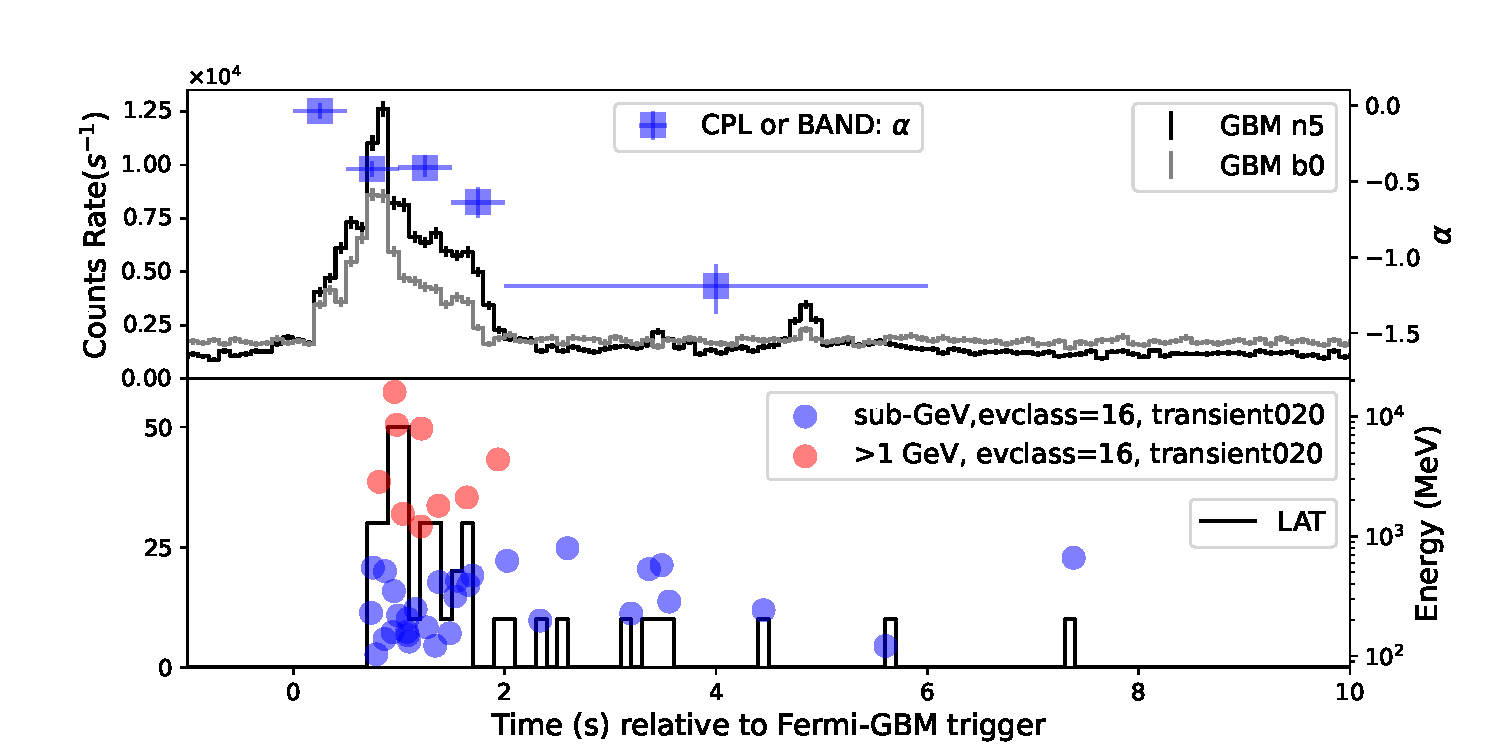
\includegraphics[width=.8\textwidth]{multi3.pdf}\put(-100,140){(a) }\\
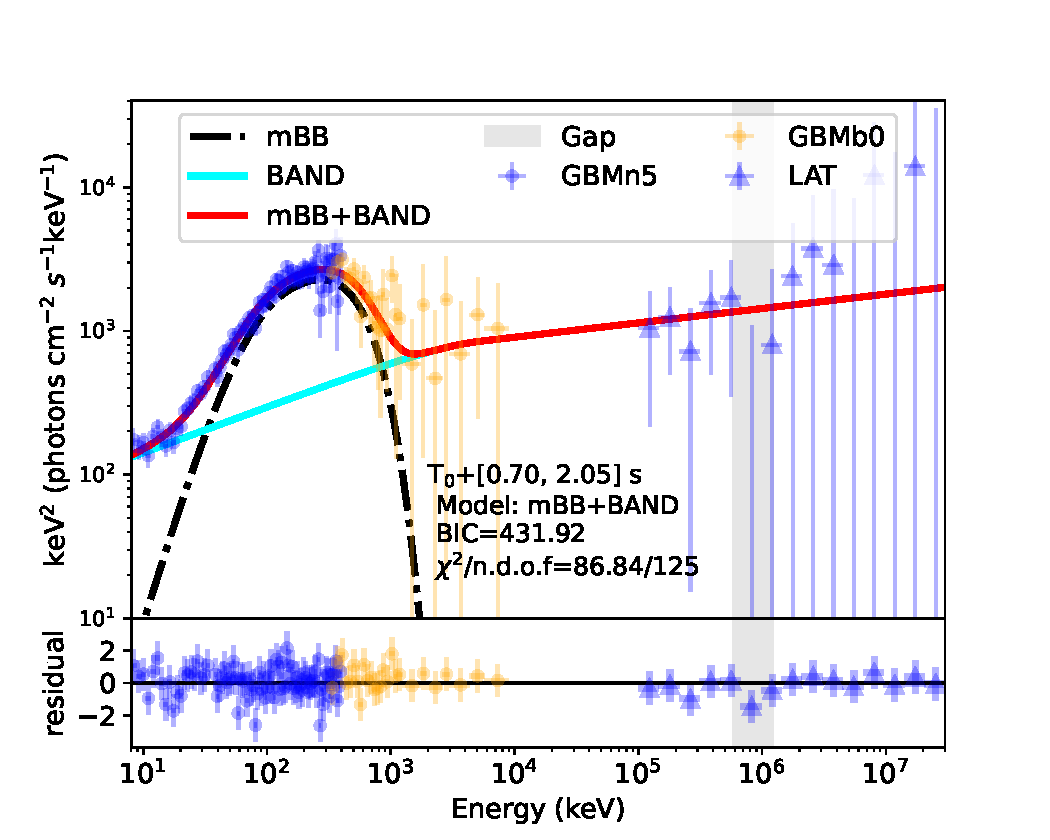
\includegraphics[width=.8\textwidth]{Fv_mBBBAND0_GRB210704A_withgapbin.pdf}\put(-110,140){(b) }
%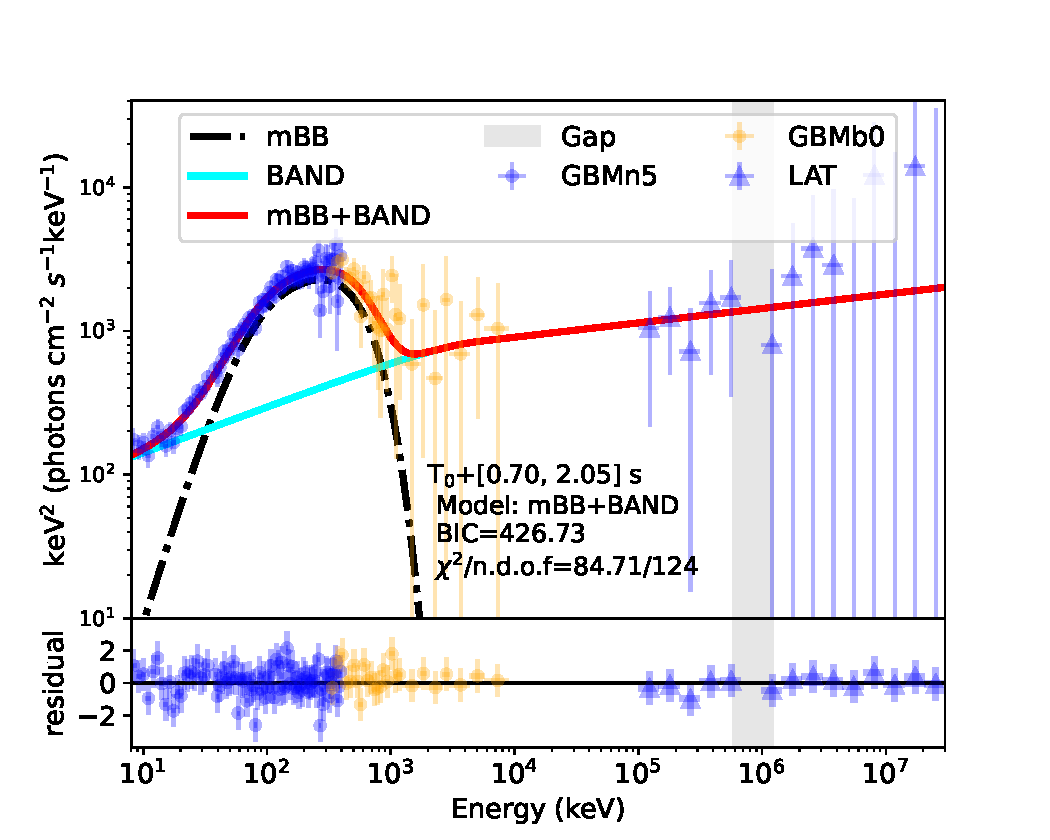
\includegraphics[width=.5\textwidth]{Fv_mBBBAND0_GRB210704A.pdf}\put(-110,140){(c) }\\
\caption{ (a) Left Y-axis with the unit of counts rate (s$^{-1}$): the histograms are the light curves of GBM detectors (NaI 5 and BGO 0, upper plot) and LAT (bottom plot); the high-energy photons are from the LAT data of TRANSIENT020 class (or evclass=16), and used in the analysis to maximize the statistics for spectral analysis of GRB prompt emission. Right Y-axis with the unit of MeV in bottom plot: energies of high-energy photons (denoted by circles). A distinct gap is observed between sub-GeV (blue circles) and GeV (red circles) photons. $\alpha$ values extracted in modeling results with the CPL (or BAND) function are denoted by blue squares with errors.
(b) The modeling results with mBB+BAND of $T_0+[0.7, 2.0]$ s, considering the 0-count bins of the gap.
%(b) and (c) are the modeling results with mBB+BAND of $T_0+[0.7, 2.0]$ s with and without considering the 0-count bins of the gap. 
 \label{fig:observation}}
 \end{center}
\end{figure*} 

\textit{The anomaly in high-energy prompt emissions.}--- The prompt high-energy emission ($>100$ MeV) peaks at $T_0+0.96$ s, with the highest-energy photon (denoted by $\gamma_{16.1 \rm GeV}$) as shown in Figure~\ref{fig:observation} (a). The light curve of the high-energy emission traces that of the MeV prompt emission almost simultaneously, or with a very small time delay, which implies that it may mainly have an internal
origin~\citep{2011MNRAS.415...77M,2012MNRAS.420..468P}. The LAT data of the TRANSIENT020 class (or evclass=16) are used in the analysis to maximize the statistics for the spectral analysis of the prompt emission of GRB.~\footnote{see the details on the web page in \href{https://fermi.gsfc.nasa.gov/ssc/data/analysis/LAT_caveats.html}{Fermi LAT caveats.}} 

From the energy distribution of the first 2 s as shown in Figure~\ref{fig:observation} (a), the upper energy envelope of sub-GeV photons begins at 0.55 GeV (denoted by
$\gamma^{\rm envelope}_{\rm sub-GeV}$) at $T_0+0.7$ s, drops to 0.25 GeV at $T_0+1.2$ s, and then increases to 0.6 GeV after $T_0+2$ s. It seems that the lower energy envelope of GeV photons (denoted by $\gamma^{\rm envelope}_{\rm GeV}$) evolves with a similar trend, while the intersection region of all gaps is observed between 0.62 GeV and 1.21 GeV.

\textit{Light curves and spectrum of prompt emission.}---
GRB 210704A has an intermediate duration, and most of the radiated energy of MeV photons is emitted in the first 2 s. Its prompt high-energy emission ($>100$ MeV) arrived almost simultaneously with the MeV emission, as shown in Figure~\ref{fig:observation} (a).

The Markov Chain Monte Carlo (MCMC) fitting is performed to find the parameters with maximum likelihood for the spectrum. The sampling tool is \textsc{emcee}~\citep{2013PASP..125..306F}.
From the modeling results with empirical functions (e.g., the BAND function and exponential cutoff power-law, i.e. CPL), the low-energy photon index ($\alpha$) of the spectra varies from 0 to -0.64 within the first 2 s, as shown in Figure~\ref{fig:observation}(a); after $T_0 +2$ s, $\alpha$ falls below -1.0.  In modeling of the spectrum of the first 0.5 s, $\alpha\simeq 0$; by the Bayesian information criterion method~\citep[BIC,][]{2016MNRAS.463.1144W}, CPL is better than the BAND function in modeling, which means the high-energy photon index $\beta\to-\infty$. This implies a typical photospheric emission in the beginning of the MeV prompt emission.
%From 0.5 to 2.0 s, although $\alpha$ is above the so-called synchrotron death-line (-2/3), there exist high-energy emissions beginning from $T_0+0.7$ s, it can hardly determine the emission mechanism only from $\alpha$~\citep[e.g.,][]{2020NatAs...4..174B}.


 
  A combined model of multicolor blackbody~\citep[mBB, e.g. see details in][]{2008ApJ...682..463P,2010ApJ...709L.172R,2018ApJ...866...13H} plus a BAND function for the broad energy band is used to describe the spectrum of prompt emission from the keV to GeV energy band;~\footnote{The parameters are listed as below for mBB+BAND, considering the 0-counts in the gap: $m=-0.37^{+0.55}_{-0.60}$, $kT_{\rm min}=18.8^{+5.8}_{-4.3}$ keV, $kT_{\rm max}=145.1^{+7.6}_{-16.8}$ keV, $F_{\rm mBB}=7.7^{+0.6}_{-0.3}\times10^{-6}$ erg cm$^{-2}$ s$^{-1}$, $\alpha=-1.68^{+0.04}_{-0.03}$, $\beta=-1.92^{+0.13}_{-0.07}$, $\log_{10}(E_{\rm p}/{\rm keV})=3.89^{+0.14}_{-0.17}$, $F_{\rm BAND}=21.7^{+2.4}_{-1.7}\times10^{-6}$ erg cm$^{-2}$ s$^{-1}$.} with a lowest BIC and the difference $\Delta \rm{BIC}>10$, it is statistically preferred over the other models (see the details in Figure~\ref{fig:spectra2} (a)-(c) in Appendix~\ref{sec:appdenix}).\footnote{\cite{2016MNRAS.463.1144W} suggested a Bayesian information criterion  (BIC$=-2\rm{ln} \mathscr{L} +\rm{ln} (N)n$, $\mathscr{L}$ denotes the likelihood
function for all these parameters based on a Bayesian prior, $\rm N$ is the number of data points, and $\rm n$ is the number of free parameters) as a tool for model selection; a model that has a lower BIC value than the others is preferred. If the change of BIC between these two models, $\Delta$BIC is from 2 to 6, the preference for the model with the lower BIC is positive; if $\Delta$BIC is from 6 to 10, the preference for that is strong; and if $\Delta$BIC is above 10, the preference is very strong.} 
  As shown in Figure~\ref{fig:observation} (b), it is evident that the component of a broad energy band has a different origin from that of the peaking component in MeV energy band. It is similar to the case of 090902B~\citep{2009ApJ...706L.138A, 2010ApJ...709L.172R, 2012MNRAS.420..468P}, therefore we think the peaking component in the MeV energy band is quasi-thermal, and this conclusion is strengthened by the physical interpretation in Section~\ref{sec:discussion}.

  For the time-integrated (TI) spectrum in $T_0+[0.7,2.0]$ s, $\Delta$BIC = 5.6 is determined for the modelings with mBB+BAND with and without considering the zero-count bins of the gap (as shown in Figure~\ref{fig:spectra2} (d) in Appendix~\ref{sec:appdenix}). This means that the preference for the model with the gap is positive.%\footnote{The parameters are listed as below
%for mBB+BAND, with considering 0-counts in the gap bins,  $m=-0.37^{+0.55}_{-0.60}$, $kT_{\rm min}=18.8^{+5.8}_{-4.3}$ keV, $kT_{\rm max}=145.1^{+7.6}_{-16.8}$ keV, $F_{\rm mBB}=7.7^{+0.6}_{-0.3}\times10^{-6}$ erg cm$^{-2}$ s$^{-1}$, $\alpha=-1.68^{+0.04}_{-0.03}$, $\beta=-1.92^{+0.13}_{-0.07}$, $log_{10}(E_{\rm p}$(keV)$)=3.90^{+0.14}_{-0.17}$, $F_{\rm BAND}=21.7^{+2.4}_{-1.7}\times10^{-6}$ erg cm$^{-2}$ s$^{-1}$;
%without considering 0-counts in the gap bins, $m=-0.37^{+0.55}_{-0.40}$, $kT_{\rm min}=18.8^{+5.6}_{-4.1}$ keV, $kT_{\rm max}=145.0^{+7.0}_{-13.4}$ keV, $F_{\rm mBB}=7.7^{+0.6}_{-0.3}\times10^{-6}$ erg cm$^{-2}$ s$^{-1}$, $\alpha=-1.68^{+0.04}_{-0.03}$, $\beta=-1.96^{+0.13}_{-0.07}$, $log_{10}(E_{\rm p}$(keV)$)=4.00^{+0.06}_{-0.21}$, $F_{\rm BAND}=19.91^{+2.4}_{-1.6}\times10^{-6}$ erg cm$^{-2}$ s$^{-1}$;} the preference for the gap in the PL model is positive.
 %The BAND function, exponential cutoff power law (CPL) and multicolor blackbody (mBB) function~\citep[e.g.][]{2008ApJ...682..463P,2010ApJ...709L.172R,2018ApJ...866...13H} (or plus on a power law (PL) component) are used to describe the time-resolved spectra in the first 2 s. By the Bayesian information criterion method~\citep[BIC,][]{2016MNRAS.463.1144W}, CPL is better than the BAND function in the modeling, and the low energy photon index ($\alpha$) varies from 0 to -0.64 within the first 2 s, as shown in Figure~\ref{fig:observation}(a); after $T_0 +2$ s, $\alpha$ falls below -1.0. The modeling of thermal emission with mBB(+PL) could describe the spectra well, especially in $T_0+1$ s to 1.5 s, the combined model of mBB+PL is the best physical model.\footnote{However, the contribution from the non-thermal part modeled with PL accounts for $\sim6\%$ of the radiative energy in this bin. Moreover, the index ($\alpha_2$) of the PL is estimated to be about -2.8; most photons are from low-energy band below 100 keV. Modelings with combined models of BB + empirical functions (BAND or CPL) are also performed, however, they are not preferred statistically than mBB (+ PL).} This implies that the prompt phase in the MeV energy band could be dominated by photospheric emission in the first 1 s; the contribution from non-thermal emission becomes larger later after $T_0+1.5$ s. The time-averaged flux in the first 2 s is about $1.0\times10^{-5}$ erg cm$^{-2}$ s$^{-1}$. %, however, due to the low statistic, the modeling with two components has considerable uncertainties. The non-thermal emission  becomes dominant from
 
 


\textit{The estimate of redshift.}--- The recent multiwavelength study of \cite{2026MNRAS.548ag555P} proposes a collapsar origin with $z=2.34$; however, \cite{2023MNRAS.522.5204B} suggest that the redshift ($z$) cannot be determined precisely from the detection: some empirical relations, e.g. the Amati relation and the EH-$T_{90}$ diagram, provide a constraint of $z>0.11$ within the $2\sigma$ level~\citep{2021GCN.30452....1M}, thus an estimate of $z<0.4$ is suggested under the assumption of a short GRB, and their analysis proposed that this burst originates from an exotic high-energy merger. In the first 0.5 s the spectrum is well described by the non-dissipative photospheric (NDP) model~\citep[e.g.,][]{2013A,Deng_2014,2022MNRAS.512.5693S,2022ApJ...931..112S}.~\footnote{The parameters extracted are listed as follows: $\log_{10} r_0=8.53^{+0.16}_{-0.25}$ cm, $\eta=217.7^{+108.8}_{-80.3}$, $\theta_c=0.13^{+0.06}_{-0.07}$ and $\log_{10} L_{\rm w}=49.77^{+0.51}_{-0.65}$, where $r_0$ is the initial radius for the outflow, $\eta$, $\theta_{\rm c}$ and $L_{\rm w}$ are the dimensionless enthalpy, the half-opening angle for the jet core and the wind luminosity, respectively; the index of the power-law index of the profile of structure jet is $p=8.5^{+6.1}_{-5.9}$, the red shift is determined to be $z=0.27^{+0.14}_{-0.12}$.}
Note that the estimated $z=0.27^{+0.14}_{-0.12}$ is extracted by NDP modeling and is model-dependent; it is consistent with the merger hypothesis. In the following, the analysis is presented with $z=0.27$, while the case of $z=2.34$ is discussed in parallel and leads to similar conclusions.





\textit{The estimate of $\Gamma$.}\label{sec:esti}---
The NDP modeling provides an estimate of $\Gamma\sim220$ with an uncertainty of about 100 from the MeV emission of the first 0.5 s. From $T_0+[0.7,2.0]$ s, $\Gamma$ could be estimated using the `top-down' approach~\citep{2015ApJ...801..103G,2024ApJ...961..137S}.\footnote{With the method described in \cite{2024ApJ...961..137S} and $Y=2$ ($Y$ is the ratio between the total outflow energy and the energy emitted; the estimated $\Gamma\propto Y^{1/4}$, thus the impact of the value of $Y$ on the estimate of $\Gamma$ is minor), all bins are found to be in the regime of $r_{\rm ra}\leq R_{\rm ph}\leq r_{\rm c}$, where $R_{\rm ph}$ denotes the photosphere radius, $r_{\rm ra}$ is the rapid acceleration radius, and $r_{\rm c}$ is the coasting radius. The estimated values of $\Gamma$ have uncertainties of about 50. The initial radius for jet launching is estimated to be $r_0\sim10^{8}$ cm.} Around the peak (from $T_0+0.7$ to $0.9$ s), the estimate of $\Gamma$ ranges between $330$ and $270$, and drops to about 190 after 1 s.
The emission of the most energetic photon ($16.1$ GeV) around the peak of luminosity requires $\Gamma \gtrsim 200$ (at a radius of $\sim10^{13}$ cm, determined in Section~\ref{sec:absorption}), with the optical depth for pair production less than unity. Thus, $\Gamma \approx 200-300$ is a reasonable value for GRB 210704A.%; in fact, the following analysis in Section~\ref{sec:discussion} on the origin of the anomaly in high-energy emission are self-consistent with this value.


%%%%%added long GRB possibilities
For $z=2.34$, $\Gamma$ is about 3.2 times that of $z=0.27$, since $\Gamma\propto\left((1+z)^2d_L\right)^{1/4}$~\citep[e.g.,][]{2007ApJ...664L...1P}. Moreover, in the following analysis, we find that the conclusions from these two possible redshifts are similar, since the comoving-frame quantities depend on $\Gamma/(1+z)$, which changes only by a factor of approximately 1.2 from $z=0.27$ to $z=2.34$.



\section{Analysis on the anomaly in prompt high-energy emission}\label{sec:ana}
\textit{The probability study of the gap.}\label{sec: probstudy}--- High-energy emission above 100 MeV could be described by a PL function. However, it is necessary to investigate whether the gaps between them could be interpreted as statistical fluctuations. 
The energy spectrum could be described by a continuous PL function with index $p$, 
\begin{equation}\label{func:PL}
N_{\rm PL}(E)=A E^{-p}.
\end{equation}
%In the modeling, $p\simeq-1.7$ and the time-averaged flux of $1.8\times10^{-5}$ erg cm$^{-2}$ s$^{-1}$ from 0.1 to 30 GeV, are determined with high-energy data from $T_0+0.7$ to 2.0 s.


A hypothesis test for the continuous PL modeling of the high-energy emission is performed, and the \textit{null hypothesis} is set to be that the statistical fluctuation could account for the gap of $[0.62,1.21]$ GeV; the test statistic is the maximum gap below an upper limit of $E_{\rm up}=1.21$ GeV. %, as listed below；
%\begin{itemize}
%    \item probabilities of the maximum gap $\mathrm{Prob_{\rm gap, max}}$;
%    \item maximum gaps below an upper limit of $E_{\rm up}=1.21$ GeV.
%\end{itemize}
A Monte-Carlo (MC) simulation is performed and $1.4\times10^5$ samples of the same total number of photons are generated based on the TI spectrum of real data in $T_0+[0.70,2.05]$ s; note that the folded model with the response from the detector is used. The probability density (PD) distribution of the maximum gaps is extracted, as shown in Figure~\ref{fig:maxEobsGeV_dTin} (a). The probability of a gap width of $\geq590$ MeV for photons below 1.21 GeV is determined to be $<10^{-3}$, thus the \textit{null hypothesis} that statistical fluctuation could explain the gap of $[0.62,1.21]$ GeV is rejected at a significance level of $\alpha=0.001$ (the corresponding $p$-value is $<10^{-3}$).


In fact, the range of the gap varies over time and in the time-integrated spectrum it is the intersection of all, which is the smallest, thus we should consider the smoothing effect of the time-integrated spectrum on the gap; the $p$-value for the gap is overestimated in the case of time-integrated analysis. %In TR analysis, the expected number of photons in the folded model in the energy bins (with index $i$) of gaps for each slice (with index $s$) is denoted as $N^{\mathrm{mod}}_{i,s}$. The probability of the gap due to the statistical fluctuation is derived as
\iffalse
\begin{equation}
\mathrm{Prob_{\rm gap}}=\prod_s \prod_i f(N^{\mathrm{mod}}_{i,s}, N^{\mathrm{obs}}_{i,s}),   
\end{equation}
\fi
%where $f(N^{\mathrm{mod}}_{i,s}, N^{\mathrm{obs}}_{i,s})$ is the Poisson probability with expected mean values of $N^{\mathrm{mod}}_{i,s}$, which are determined by modeling. Note that in the modeling, the energy bins, including the zero-count bins in gaps, are all used, thus $\rm Prob_{\rm gap}$ is determined conservatively. 
Similar procedures are performed in the time-resolved analysis, with the spectral index fixed to that of the time-integrated modeling. As shown in Table~\ref{tab:gapprob}, the lowest $p$-value is $6\times10^{-4}$ in $T_0+[0.9, 1.2]$ s, which is less than that of the time-integrated analysis; the product of the sequence of $p$-values ($\prod p$-value) is very tiny ($\ll10^{-6}$) considering the width of the gap that changes over time.

In addition, a full likelihood analysis performed with \textsc{gtlike} corroborates this conclusion: comparing the continuous PL model with a model explicitly incorporating a spectral gap of $[0.6, 1.2]$ GeV\footnote{For \textsc{gtlike}, a ``FileFunction'' option is allowed for a fixed spectral shape and the sole parameter is a multiplicative normalization. To obtain the best parameter for the PL with a gap of 0.6 to 1.2 GeV, a parameter scan is performed for the index of the power law, and the minimum $-\log(\rm likelihood)$ and the error (the difference between the index of the minimum $-\log(\rm likelihood)$ and that of $-\log(\rm likelihood)\pm0.5$) are extracted.} yields a preference for the model with the gap, with $\Delta \mathrm{BIC}=-2\Delta\log(\rm likelihood)=9.2$, which constitutes strong statistical evidence against a simple continuous spectrum.

\begin{figure*}
\begin{center}
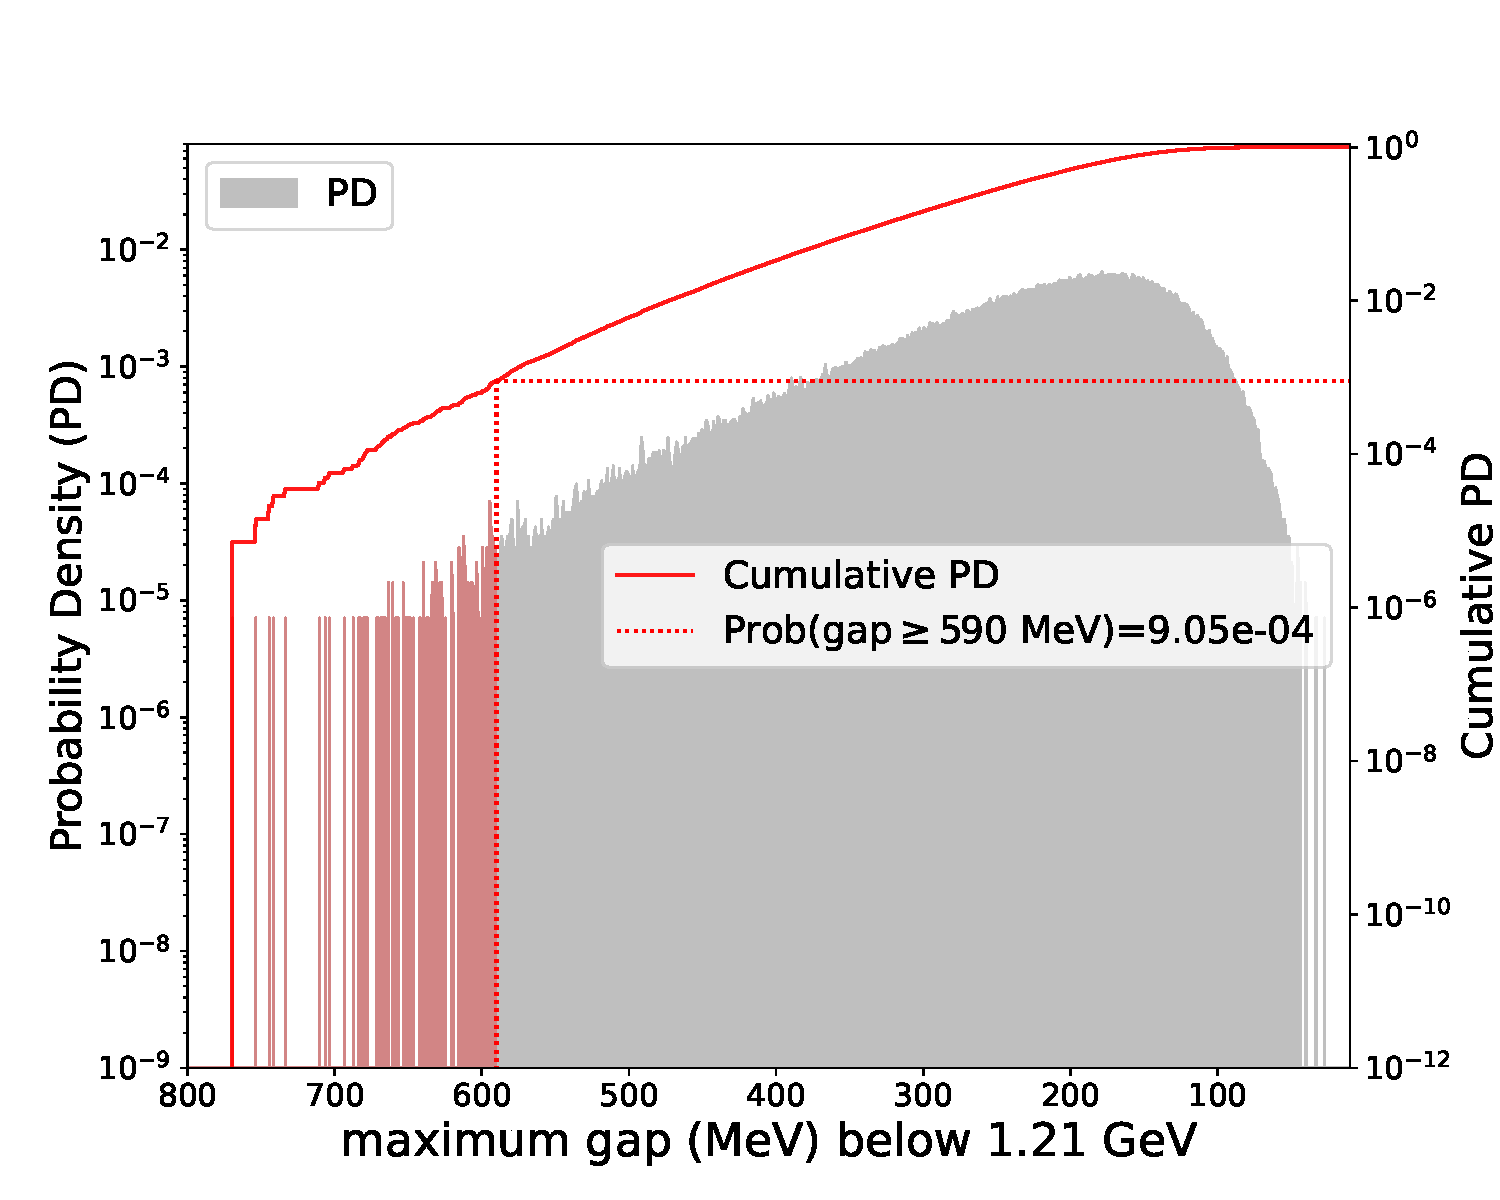
\includegraphics[width=.5\textwidth]{gapdis_hist_siglevel.pdf}\put(-80,160){(a) }
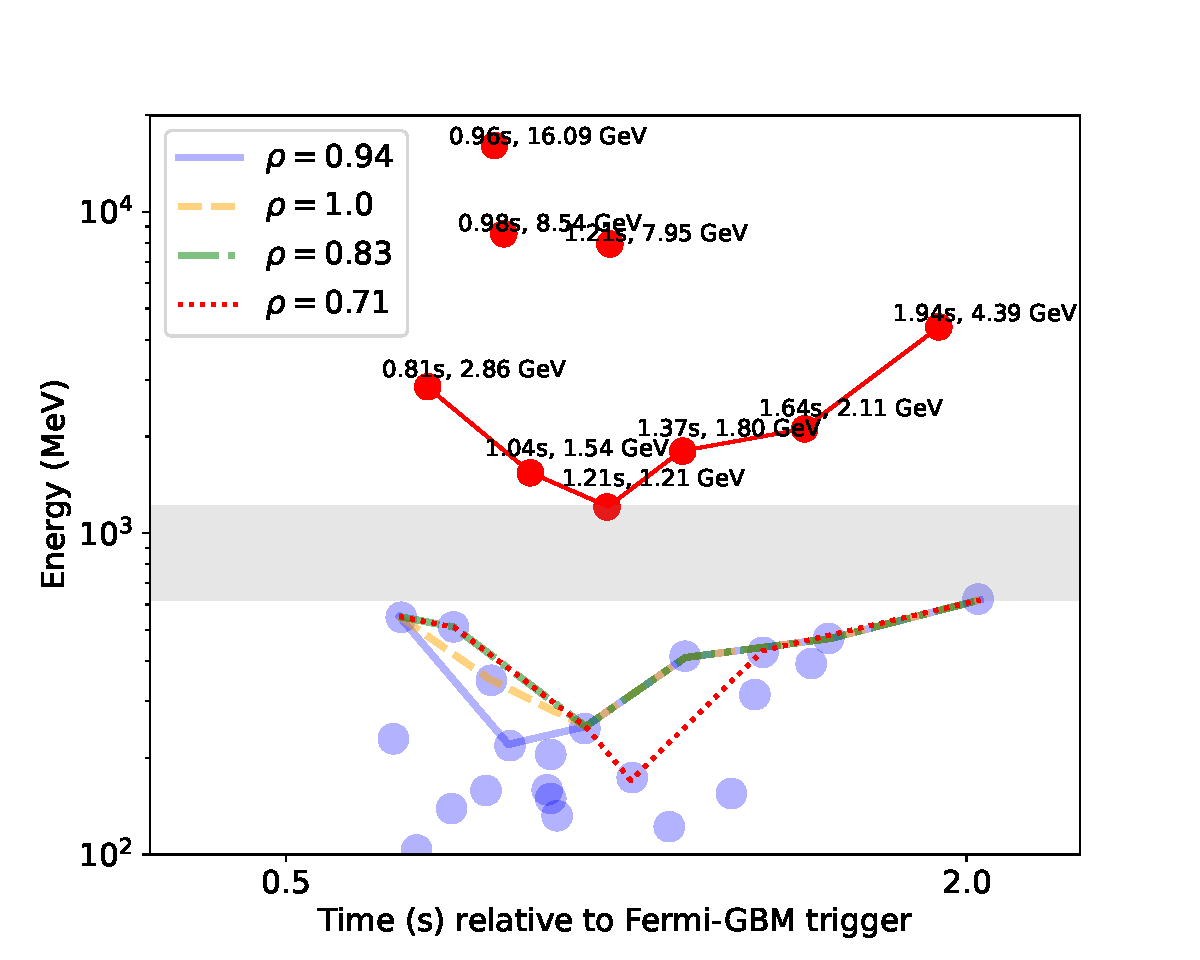
\includegraphics[width=.5\textwidth]{EvsT_LAT0p5_2p2_2.pdf}\put(-80,160){(b) }\\
%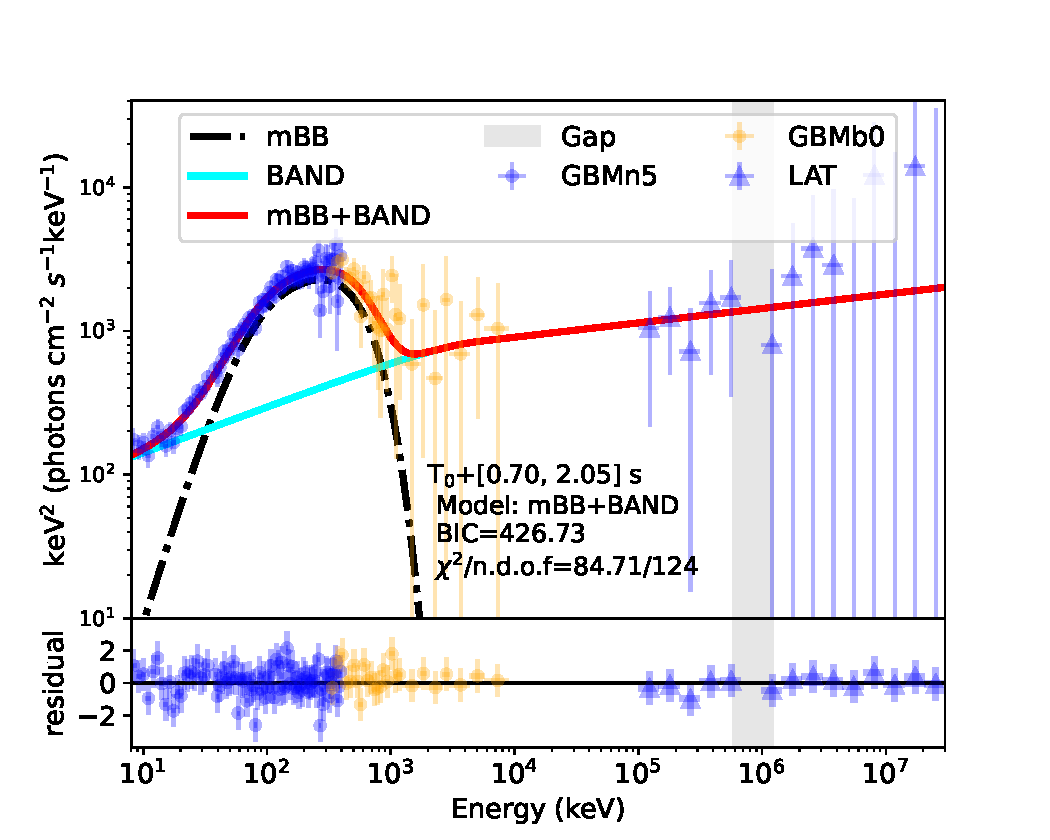
\includegraphics[width=.5\textwidth]{Fv_mBBBAND0_GRB210704A.pdf}%{Fv_PL0_GRBHEB210704.pdf}\put(-50,160){(c) }\\
\caption{ (a) PD (the gray shadow) of maximum gaps in photons below 1.21 GeV and cumulative PD (the solid red line). The $p$-value of the maximum gap $\geq 590$ MeV is labeled by the dotted red line, which is determined by the cumulative PD in red shadow.(b) The Spearman rank correlation coefficients ($\rho$) of temporal evolution between $\gamma^{\rm envelope}_{\rm GeV}$ and $\gamma^{\rm envelope}_{\rm sub-GeV}$ (denoted by different line styles and colors) extracted with different bin-edge division ratios. The gray shadow between [0.62, 1.21] GeV shows the intersection of all gaps between sub-GeV and GeV photons. % (c) The spectral modeling with and without the gap bin. 
\label{fig:maxEobsGeV_dTin}}
 \end{center}
\end{figure*} 

\begin{deluxetable*}{lccccc}
%\tabletypesize{\tiny}
%\tabletypesize{\small}
\tablewidth{0pt}
\tablecaption{Time-resolved gaps and $p$-values.\label{tab:gapprob}}
\tablehead{ 
\colhead{Time bins (s)}
&\colhead{[0.70, 0.90]}
&\colhead{[0.90, 1.20]}
&\colhead{[1.20, 1.40]}
&\colhead{[1.40, 1.65]}
&\colhead{[1.65, 2.05]}
%&\colhead{$\prod_s \prod_i f(N^{\mathrm{mod}}_{i,s}, N^{\mathrm{obs}}_{i,s}=0)$}\\
\\
\colhead{Gap range (MeV)}&\colhead{[2860, 550]}&\colhead{[1540, 350]}&\colhead{[1210, 410]}&\colhead{[2110, 430]}&\colhead{[4390, 620]}
}
\startdata
% index $p$ fixed to TI results & & &$1.74\pm{0.10}$&&&\\
 $p$-value &0.0037 &0.0006 &0.0180 &0.0067 &0.0034 \\\hline
%$N^{\mathrm{mod}}_{i,s}$, $f(N^{\mathrm{mod}}_{i,s},N^{\mathrm{obs}}_{i,s}= 0)$ of gap  &2.23,0.107&4.9,0.007&1.99,0.137&1.68,0.186&1.51,0.22&$4.5\times10^{-6}$\\
%$N^{\mathrm{mod}}$ and $f$  above GeV-line &0.72,0.489&2.38,0.262&1.61,0.322&0.64,0.525&0.3,0.741&$1.6\times10^{-2}$\\\hline
\enddata
\end{deluxetable*}


\textit{The possible correlation between  $\gamma^{\rm envelope}_{\rm sub-GeV}$ and $\gamma^{\rm envelope}_{\rm GeV}$.}\label{sec: correlation}---The Spearman rank correlation coefficient ($\rho$)~\citep{spearman}\footnote{The spearman rank correlation coefficient $\rho$ is defined as $\rho = \frac{\mathrm{cov}(r(x),r(y))}{\sigma_x \sigma_y} $ where $r(a)$ represents the rank of element $a$. For non-duplicated datasets, $\rho$ can be interpreted as $\rho = 1 - \frac{6 \Sigma d^2_i}{n(n^2-1)} $ where $d_i = r(x) - r(y)$.} is used to quantify the monotonic relationship of the temporal evolution between the energy of $\gamma^{\rm envelope}_{\rm GeV}$ and that of $\gamma^{\rm envelope}_{\rm sub-GeV}$. $\gamma^{\rm envelope}_{\rm GeV}$ is naturally formed by the GeV photons as shown in Figure~\ref{fig:maxEobsGeV_dTin} (b) in red circles connected by a red line. In order to ensure a one-to-one correspondence between $\gamma^{\rm envelope}_{\rm sub-GeV}$ and $\gamma^{\rm envelope}_{\rm GeV}$, the maximum sub-GeV energy value in each time bin was extracted as the energy envelope of sub-GeV photons; the data binning in the range of $T_0+[0.7, 2.0]$ s is performed as follows: 1) the bin edges are determined to be the n-equal diversion points in time of each adjacent GeV point in $\gamma^{\rm envelope}_{\rm GeV}$; 2) to reduce the impact of artificial selection, the bin-edge division ratio (rate) is tested from 0.01 to 0.99 with an increment of 0.01 (for example, a rate equal to 0.2 means left five-division point).  

From all binning results with different bin-edge division ratios, four different energy envelopes of sub-GeV photons were extracted, as shown in Figure~\ref{fig:maxEobsGeV_dTin} (b). $\rho$ is determined to be $> 0.7$ conservatively from the results of all sets of bin edges, which implies a strong correlation between $\gamma^{\rm envelope}_{\rm sub-GeV}$ and $\gamma^{\rm envelope}_{\rm GeV}$.\footnote{The grading standards and the corresponding correlation degrees are available online:~\href{https://www.statstutor.ac.uk/resources/uploaded/spearmans.pdf}{Spearman's correlation}. }

%\textit{TI spectral modeling with and without gap.}\label{sec: modeling}--- The gap is statistically significant as analyzed in Section~\ref{sec: probstudy}. To further confirm this conclusion, modelings are performed with and without considering the gap in the model. However, the statistic is not large enough to extract the parameters of a specific physical model (e.g., an absorption line described by a gaussian function); moreover, the center energy and width of the gap vary with time, as shown in Fig~\ref{fig:observation} (c). Thus, the result of modeling with the gap subtracted in the bin is compared with that of all bins.
%The Markov Chain Monte Carlo (MCMC) fitting is performed to find the parameters with maximum likelihood. The Sampling tool is $emcee$~\citep{2013PASP..125..306F}. \cite{2016MNRAS.463.1144W} suggested a Bayesian information criterion (BIC$=-2\rm{ln} \mathscr{L} +\rm{ln} (N)n$, $\mathscr{L}$ denotes the likelihood function for all these parameters based on a Bayesian prior, $\rm N$ is the number of data points, and $\rm n$ is the number of free parameters) as a tool for model selection; a model that has a lower BIC value than the others is preferred. 
%As shown in Figure~\ref{fig:maxEobsGeV_dTin} (b), the extracted indices of PL function are similar in the modelings with and without the gap; $\Delta$BIC=4.2, the preference for the gap in the PL model is positive.\footnote{If the change of BIC between these two models, $\Delta$BIC is from 2 to 6, the preference for the model with the lower BIC is positive; if $\Delta$BIC is from 6 to 10, the preference for that is strong; and if $\Delta$BIC is above 10, the preference is very strong.}




  

\section{The physical interpretation}\label{sec:physical_interpretation}
%To account for the gap and correlation between $\gamma^{\rm envelope}_{\rm sub-GeV}$ and $\gamma^{\rm envelope}_{\rm GeV}$, some physical interpretations could be proposed naturally: sub-GeV photons and GeV photons are not produced from the same mechanism (see the details in Section~\ref{sec: multi}); or the photons produced between $\gamma^{\rm envelope}_{\rm sub-GeV}$ and $\gamma^{\rm envelope}_{\rm GeV}$, are absorbed by some resonant nuclide or photon-photon pair production (see the details in Section~\ref{sec:absorption}). %In order to distinguish between possible interpretations, an estimate of $\Gamma$ is given in Section~\ref{sec:esti}.


 %A model-dependent approach~\citep[e.g.,][]{2015ApJ...801..103G,2024ApJ...961..137S} is performed to obtain the estimate of the Lorentz Factor. For GRB 210704A,
 

\subsection{The multi-component emission mechanism, or a two-component jet model ?}\label{sec: multi}
 %If the GeV photons are due to another mechanism that differs from that of sub-GeV photons, the evolution of $\Gamma$ may account for the correlation between $\gamma^{\rm envelope}_{\rm sub-GeV}$ and $\gamma^{\rm envelope}_{\rm GeV}$, since the energies of $\gamma^{\rm envelope}_{\rm sub-GeV}$ and $\gamma^{\rm envelope}_{\rm GeV}$ are both boosted with the same Lorentz Factor. 

 The scenario in which GeV photons are produced by the re-scattering of sub-GeV photons via the inverse Compton (IC) mechanism can hardly account for the energy difference. In the Thomson regime, one has
\begin{equation}
E_{\rm IC, obs}\simeq\Gamma\gamma'^{2}_e E'_{\rm seed}/(1+z),    
\end{equation}
 where the energy ratio of the re-scattered photons to the sub-GeV ones that are only scattered once is $\gamma_e^{'2}$; $\gamma_e^{'2}$ is estimated to be about 5 from the observations of (2.86 GeV, 0.55 GeV) and (1.21 GeV, 0.25 GeV). For the production of sub-GeV photons, $E'_{\rm seed}\sim 500$ keV is too energetic for seed photons in the comoving frame and the Thomson regime.
 In the Klein-Nishina (KN) regime, re-scattered photons cannot gain more energy via multi-time scattering. 
 %Thus, multi-scattering can hardly explain the anomaly.

 A two-component jet model~\citep[a fast spine and slow sheath, e.g. see][]{2025ApJ...995L...2A} fails to explain the synchronized temporal evolution of the sub-GeV and GeV components. Therefore, we turn to photon-matter interactions.

 



 
 


\subsection{The Resonant Nuclide Absorption Scenario and Other Potential Absorption Mechanisms}
\label{sec:resonant-nuclide-absorption}\label{sec:absorption}

\textit{Energy scale.}---Applying the Doppler correction $E' \approx E_{\rm obs} (1+z) / 2\Gamma$, the observed gaps translate to a comoving energy range of:
\begin{equation}
E_{\rm gap}^{\prime} \approx 2 - 7 \text{ MeV}.
\end{equation}
Note that for $z=2.34$ the correspondingly larger $\Gamma$ leads to a similar range, since $\Gamma/(1+z)$ changes only by a factor of about 1.2 (see Section~\ref{sec:obs}).

%where the lower (upper) limit corresponds to 0.55 (2.86) GeV and $\Gamma\simeq 280$(260). 
We propose that the gap arises from the resonant absorption of photons by nuclei entrained in the jet. The comoving energy of $\sim 4$ MeV aligns remarkably well with the photodissociation threshold of deuterium:
\begin{equation}
\gamma + {^2\text{H}} \rightarrow p + n.
\end{equation}
The binding energy of deuterium is 2.22 MeV. However, the cross-section for photodissociation peaks slightly above the threshold, typically around $4-5$ MeV \citep{IAEA2000}, which perfectly matches our derived comoving energy $E_{\rm gap}^{\prime}$.

Crucially, this energy scale distinguishes deuterium from all other potential nuclear absorbers. Heavier nuclides, particularly the Fe-group elements often invoked in supernova models, interact with photons primarily through the Giant Dipole Resonance (GDR). The GDR peak energy for nuclei with mass number $A$ is approximately $E_{\rm GDR} \approx 31.2 A^{-1/3} + 20.6 A^{-1/6}$ MeV \citep{1975RvMP...47..713B}, which places the resonance at $15-25$ MeV for heavy elements (e.g., $^{56}$Fe) \citep{2020NuDS..163..109K}. Such an absorption would manifest at observed energies $>3$ GeV, far above the gap detected in GRB 210704A. The unique low-energy threshold of deuterium makes it the only viable candidate for an absorption feature at $\sim 4$ MeV.

\textit{Timescales and Nucleosynthesis.}---The identification of deuterium is further supported by the dynamical timescales of the GRB jet. %ref
With the standard internal shock model for the prompt emission, the emitting radius is~\citep{2011ApJ...726...90Z}
\begin{equation}\label{eq:Ris}
R \simeq 2 \Gamma^2 c \delta t/(1+z) \simeq 6 \times 10^{12} \Gamma_{2.5}^2 \delta t_{-3}/(1+z) \ {\rm cm},
\end{equation}
where $\delta t$ is the timescale of the pulse duration; hereafter, the convention $Q_s = Q/10^s$ is adopted in cgs units throughout the text. $\delta t$ is determined to be about 1 ms by a wavelet decomposition of the light curve of the internal shock emission (photons with energies $< 20$ keV are required, and the contribution from the quasi-thermal emission is $7\%$; the light curve has a sampling rate of 4000 Hz; see the details of the method in~\citealt{2013MNRAS.432..857M}). The emitting radius is thus of the order of $10^{12}-10^{13}$ cm, a typical value for short GRBs~\citep{2014ARA&A..52...43B}. The dynamical time in the comoving frame is then extremely short, only a fraction of a second:
\begin{equation}
t'_{\rm dyn} \approx \frac{R}{\Gamma c} \sim 0.1 R_{12} \Gamma_{2.5}^{-1} \text{ s}.
\end{equation}
In a neutron-rich outflow ejected from a merger, nucleosynthesis begins with the rapid capture of neutrons by protons ($p + n \rightarrow {^2\text{H}}$). To form heavier r-process elements (up to lanthanides), the chain must proceed through seed nuclei creation. However, the formation of seeds heavier than deuterium is rate-limited by weak interactions ($\beta$-decays), which typically require timescales of seconds to minutes to proceed significantly; a fraction of a second is far too short for heavier elements to form.

Given the relativistic expansion, the jet material is ``frozen out" before significant quantities of heavy elements can form via $\beta$-decay. Consequently, the jet composition at the photospheric radius is expected to be dominated by nucleons and light isotopes, specifically deuterium, rather than heavy metals. This kinetic constraint robustly excludes Fe-group elements and reinforces the deuterium interpretation.



\textit{Other candidate absorption mechanisms.}---As another candidate absorption mechanism, photon-photon pair production ($\gamma+\gamma \to
e^+ + e^-$) could in principle attenuate the high-energy spectrum; however, its optical depth increases monotonically with the photon energy above the threshold, so it would produce a high-energy cutoff rather than a discrete gap followed by a recovery in flux above 1.21 GeV. Moreover, to generate an observed absorption with a center energy of $\sim1$ GeV, pair production requires a much larger Lorentz factor, e.g. $\Gamma\gtrsim 1000$, than the estimate. Therefore, it is unlikely unless there exists sufficient evidence for an extremely large Lorentz factor.


\section{Discussion and Conclusion}\label{sec:discussion}

\textit{Discussion.}--- The comoving density of the jet, mainly contributed by protons, is expressed in terms of the isotropic kinetic energy of the jet $E_{\rm K}$ at the emission radius $R$ as~\footnote{In the comoving frame, the shell volume is $V'=4\pi R^2 (R/\Gamma)$; one has $n^{\prime}_{p}V'm_pc^2=M_{\rm iso}c^2$ and $E_{\rm K}=\Gamma M_{\rm iso} c^2$.}
\begin{eqnarray}\label{eq:nbp}
 n^{\prime}_{p}&=&\frac{E_{\rm K}}{4\pi R^3 m_p c^2}\nonumber\\
     &=&1.7\times 10^{17} E_{\rm K,53} R_{12.5}^{-3} \ \rm cm^{-3} , \nonumber\\
\end{eqnarray}
where $E_{\rm K,53}=E_{\rm K}/10^{53}$ erg and the unit of $R$ is cm. The comoving density of deuterium $n'_{D}$ is estimated with the number fraction of deuterium ($Y_{D}$) to be:
\begin{equation}\label{eq:nDp}
   n^{\prime}_{ D}= 0.1 n^{\prime}_{p} Y_{D,-1}.
\end{equation}
The optical depth for the photodissociation of deuterium is 
\begin{equation}
  \tau_{\gamma D}\sim\frac{\sigma_{\gamma D} n'_ D R}{\Gamma}=1.3 E_{\rm K, 53} R_{12.5}^{-2} Y_{D,-1} \Gamma_2^{-1},
\end{equation}
where $\sigma_{\gamma D}\simeq 2.5\times10^{-27}$ cm$^{2}$ at a photon energy
$\varepsilon'_\gamma \simeq 4.48~{\rm MeV}$ in the deuteron rest frame \citep{IAEA2000}.


Internal shocks are natural sites for the dissipation of the kinetic energy of a baryonic fireball~\citep[][]{1990ApJ...365L..55S,1992MNRAS.258P..41R,1993ApJ...405..278M,1994ApJ...430L..93R}.
In the internal shock model of gamma-ray bursts, electrons accelerated at mildly relativistic shocks are commonly assumed to follow a non-thermal distribution \citep{2004RvMP...76.1143P},
\begin{equation}
N(\gamma_e) \propto \gamma_e^{-p}, \qquad \gamma_e \ge \gamma_m ,
\end{equation}
where $\gamma_m$ is the minimal Lorentz factor of the electrons accelerated in the internal shocks.
For typical internal shock parameters adopted in the literature, $\gamma_m \sim 10^{3.5}$--$10^6$ \citep{2013ApJ...769...69B,2019A&A...628A..59O}. The scattering regime between photons and relativistic electrons is determined by
\begin{equation}
x \equiv \frac{\gamma_e \varepsilon'_\gamma}{m_e c^2},
\end{equation}
where $\varepsilon'_\gamma$ is the photon energy in the comoving frame. One has $x \gtrsim 2.5\times 10^4$ for $\varepsilon_\gamma'=4$ MeV and $\gamma_m\gtrsim10^{3.5}$. In this Klein-Nishina limit, the total scattering cross section is suppressed to \citep{1986rpa..book.....R}
\begin{equation}
\sigma_{\rm KN} \simeq 
\frac{3}{8}\sigma_T
\frac{\ln(2x)+1/2}{x} 
\lesssim 1.1 \times 10^{-28} {\rm cm}^2,
\label{eq:sigmaKN-GBM}
\end{equation}
thus, the optical depth for Compton scattering in the Klein-Nishina regime is 
\begin{equation}
\tau_{\rm KN} \sim \frac{\sigma_{\rm KN} n'_e R}{\Gamma}
\lesssim 0.6 E_{\rm K, 53}R_{12.5}^{-2} \Gamma_2^{-1},
\label{eq:tauKN-GBM}
\end{equation}
assuming local electric neutrality in the jet, $n'_{e}\simeq n'_p$. The break energy ($\varepsilon_b$) in the spectrum of the non-thermal component described by a BAND function (e.g. the synchrotron emission by the relativistic electrons in magnetic field) may correspond to $\tau_{\rm KN} (\varepsilon_b')\sim1$ at $\gamma_e=\gamma_m$. From the results of the modeling of the non-thermal component, the break energy is $\varepsilon_b\sim10^4$ keV, which corresponds to $\gamma_m\sim10^{5.4}$ in this case; $\sigma_{\rm KN}\sim10^{-30}$ cm$^{2}$ is much lower for the photons of $\varepsilon_\gamma'=4$ MeV, due to a deeper Klein-Nishina regime.





Let us demonstrate
the plausibility of the observation of photodissociation of deuterium in the jet of GRB 210704A as follows: the first key point is whether the baryon loading in the relativistic outflow could produce enough deuterium;
second, GeV photons are emitted while those in the resonant region are absorbed by deuterium, which requires that $\tau_{\gamma D}$ and $\tau_{\rm KN}$ (for GeV photons) satisfy
\begin{equation}\label{eq:criterion}
    \tau_{\rm KN}<1\lesssim\tau_{\gamma D}.
\end{equation}
The freezeout $Y_{D}$ can be greater than a few percent or even as large as $10\%$ under the right conditions below the radius of GeV emissions \citep[see the simulation in][]{2002ApJ...580..368P}; the production of deuterium could be further enhanced through the spallation of $\alpha$-particles~\citep{2003ApJ...588..931B}, which is caused by neutron-ion decoupling as well as internal shocks. Therefore $\tau_{\gamma D}$ could be larger than $\tau_{\rm KN}$ in this case. The total energy of the outflow could be estimated from the radiated energy $E_{\gamma, \rm iso}$ and the radiative efficiency ($\epsilon_\gamma$) as
\begin{equation}
    E_{\rm tot, iso}= E_{\gamma, \rm iso}/\epsilon_\gamma;
\end{equation}
for baryonic fireball, $E_{\rm K}\lesssim (1-\epsilon_\gamma)E_{\rm tot, iso}$.
It is reasonable that $\epsilon_\gamma\lesssim10\%$, because the radiation efficiency of internal shocks is typically low~\citep[][]{2011ApJ...726...90Z,2008FrPhC...3..306F}. $E_{\gamma, \rm iso}\simeq 10^{52}$ erg for GRB 210704A, thus we assume that $E_{\rm K}$ is comparable to $10^{53}$ erg, or even several times larger. The internal shock radius (Eq.~\ref{eq:Ris}) has an order of magnitude of $10^{12}-10^{13}$ cm. Thus, given $Y_{D}\simeq0.1$, $E_{\rm K}\sim10^{53}$ erg and $R\sim10^{12.5}$ cm, Eq.~(\ref{eq:criterion}) is satisfied. The baryon loading in the jet is calculated to be $f_{b}M_{\rm iso}\sim10^{-6}M_{\odot}$ by $E_{\rm K}=\Gamma M_{\rm iso}c^2$ (the typical beaming factor for short GRBs is $f_b\sim6\times10^{-3}$~\citep[][]{2014ARA&A..52...43B}), which is a reasonable value for merger events~\citep{2019LRR....23....1M,2025PhRvD.111f3040S}.



\textit{Conclusion.}---
We identified a statistically significant spectral gap in the prompt emission of GRB 210704A. Interpreting this for the first time as resonant absorption by deuterium nuclei entrained in the relativistic jet, we find a consistent physical picture that links the burst to a neutron-rich outflow. This represents the first direct spectroscopic detection of r-process nucleosynthesis ingredients in the prompt gamma-ray phase, opening a new window for studying nuclear astrophysics in extreme environments.
%We identified a statistically significant spectral gap in the prompt emission of GRB 210704A. Interpreting this as resonant absorption by deuterium nuclei in a jet with $\Gamma \sim 200-300$ for the first time, we find a consistent physical picture that links the burst to a neutron-rich progenitor.


Previous studies of GRB 210704A noted its peculiar properties, with its duration lying in the intermediate range; both a compact-object merger origin \citep{2021GCN.30380....1M, 2023MNRAS.522.5204B} and a collapsar origin \citep{2026MNRAS.548ag555P} have been proposed. Unlike kilonovae, which probe the sub-relativistic ejecta days after the event, this spectral feature probes the relativistic jet itself seconds after launch, revealing the initial chemical composition of the r-process flow. It should be noted that such observations are expected to be rare: GRB 210704A is a `short' long burst that favors the abundance of deuterium, and the high baryon loading of the outflow together with the rapid variability of the central engine creates the conditions for the occurrence of intense internal shocks.
%Previous studies of GRB 210704A noted its peculiar properties and suggested a compact object merger origin, despite its duration lying in the intermediate range \citep{2021GCN.30380....1M, 2023MNRAS.522.5204B}. Our finding provides a completely independent confirmation of this progenitor channel.
%TC:ignore
%\iffalse
\begin{acknowledgements}
 The authors are very grateful for the public GRB data from Fermi/GBM and Fermi/LAT. Dr. X.Y. Song thanks the support of the National Natural Science Foundation of China (grant No.12303052). Q. Liu and Dr. X.Y. Song are very grateful for the support from China's Space Origins Exploration Program. Prof. B.Q. Ma and Q. Liu appreciate the support of the National Natural Science Foundation of China (grant No.12335006). The authors thank anonymous reviewers for their useful comments. The authors thank Prof. Shuang-Nan Zhang, Prof. Ming-Yu Ge, and Prof. Francesco Longo for useful comments and discussions on the data analysis.
\end{acknowledgements}
\appendix
\section{Spectral modelings with different models}\label{sec:appdenix}
The modeling results with the other models, including BAND, BB+BAND and mBB+PL, are shown in Figure~\ref{fig:spectra2} (a)-(c). The modeling result with mBB+BAND without the zero-count bins in the gap is shown in Figure~\ref{fig:spectra2} (d).
\begin{figure*}
\begin{center}
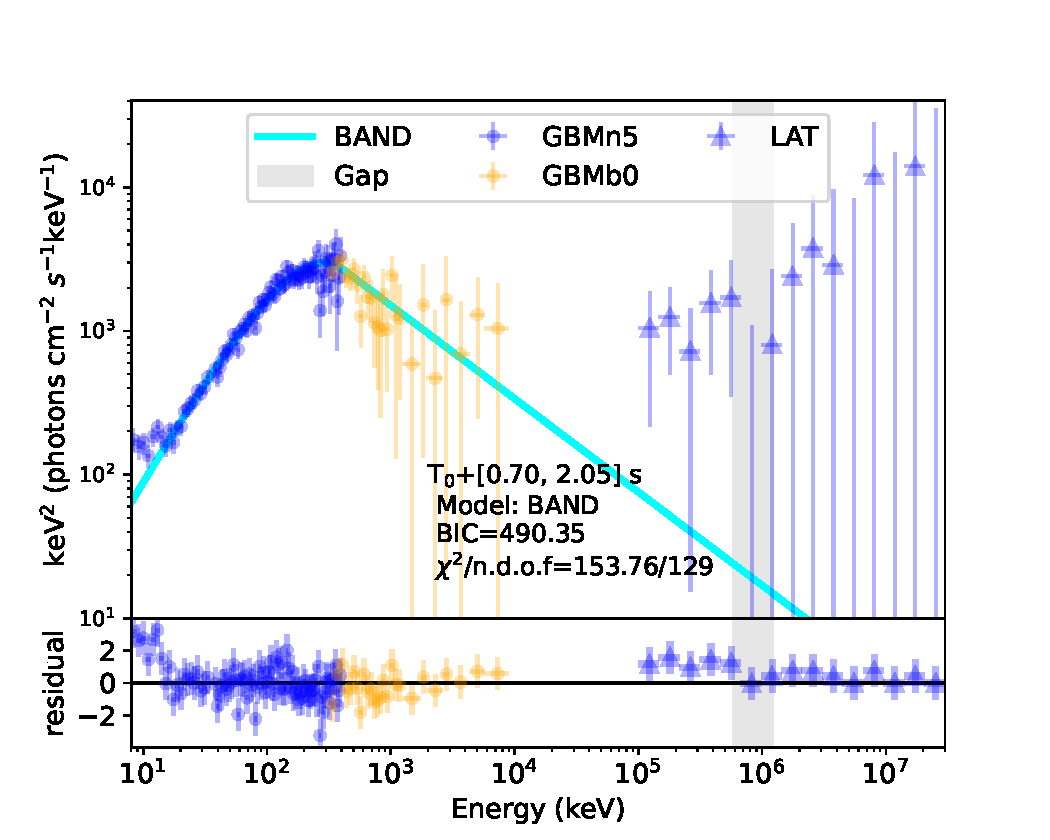
\includegraphics[width=.5\textwidth]{Fv_BAND0_GRB210704A.pdf}\put(-100,140){(a) }
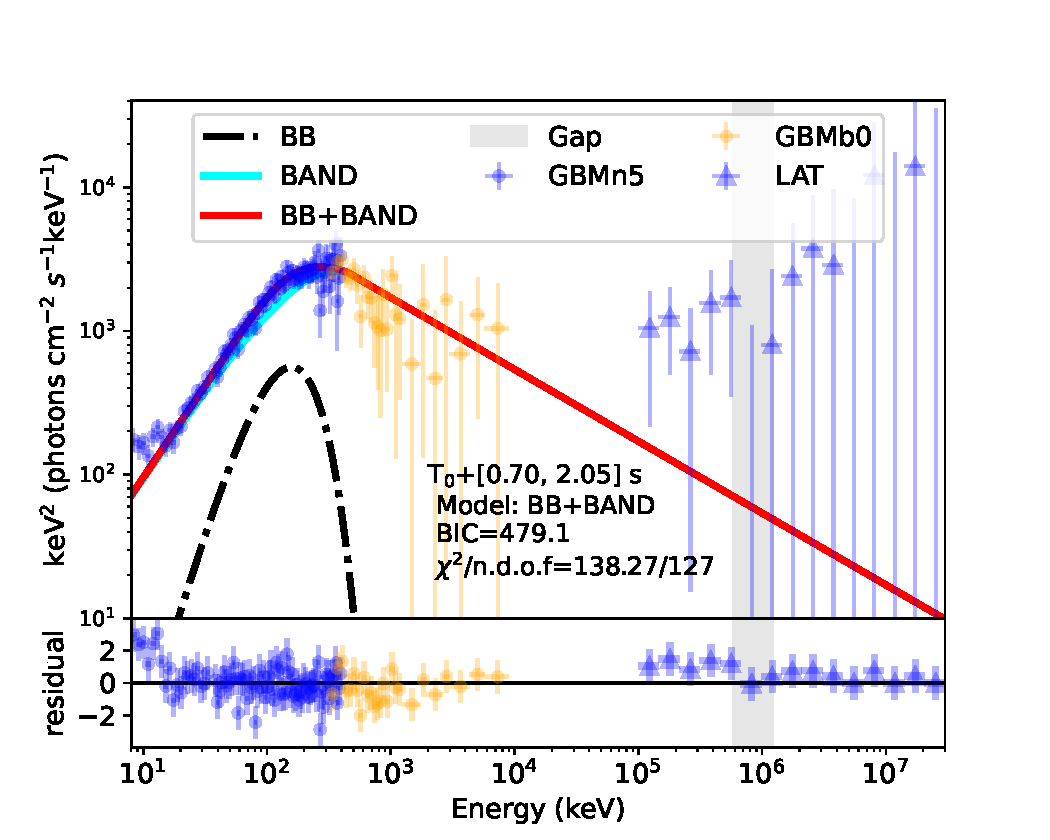
\includegraphics[width=.5\textwidth]{Fv_BBBAND0_GRB210704A.pdf}\put(-80,140){(b) }\\

%\includegraphics[width=.5\textwidth]{Fv_mBBbPL0_GRB210704A.pdf}\put(-60,160){(d) }
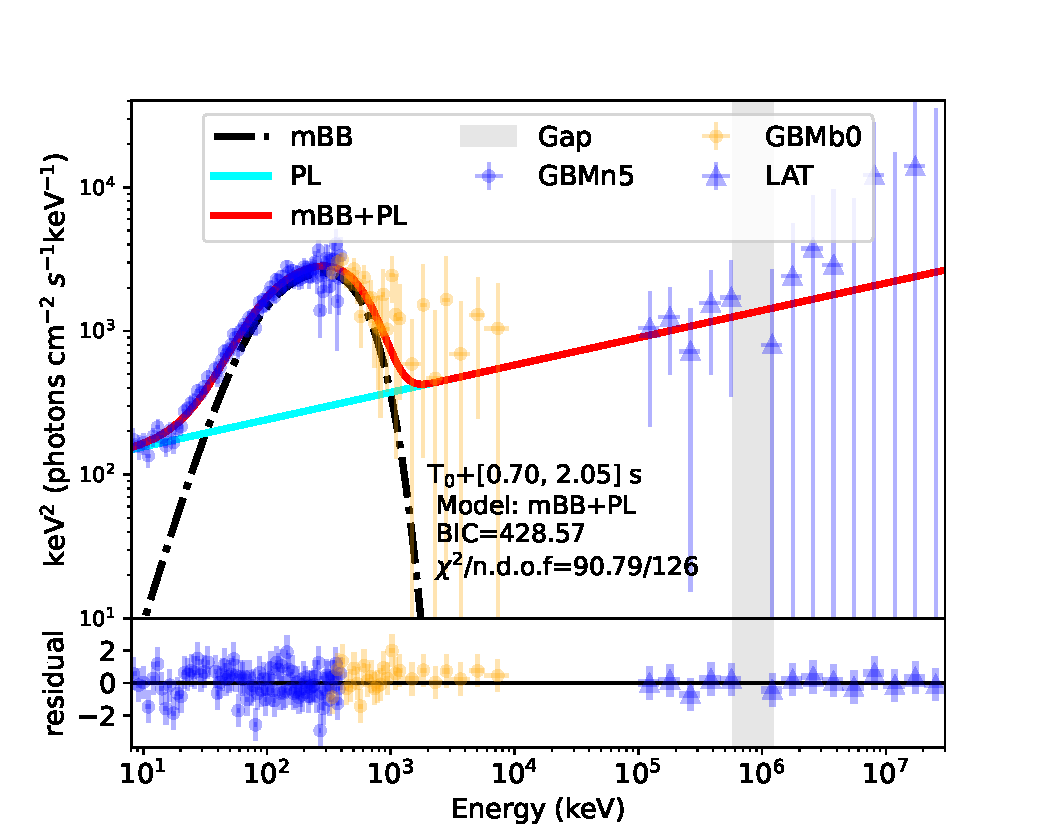
\includegraphics[width=.5\textwidth]{Fv_mBBPL0_GRB210704A.pdf}\put(-90,140){(c) }
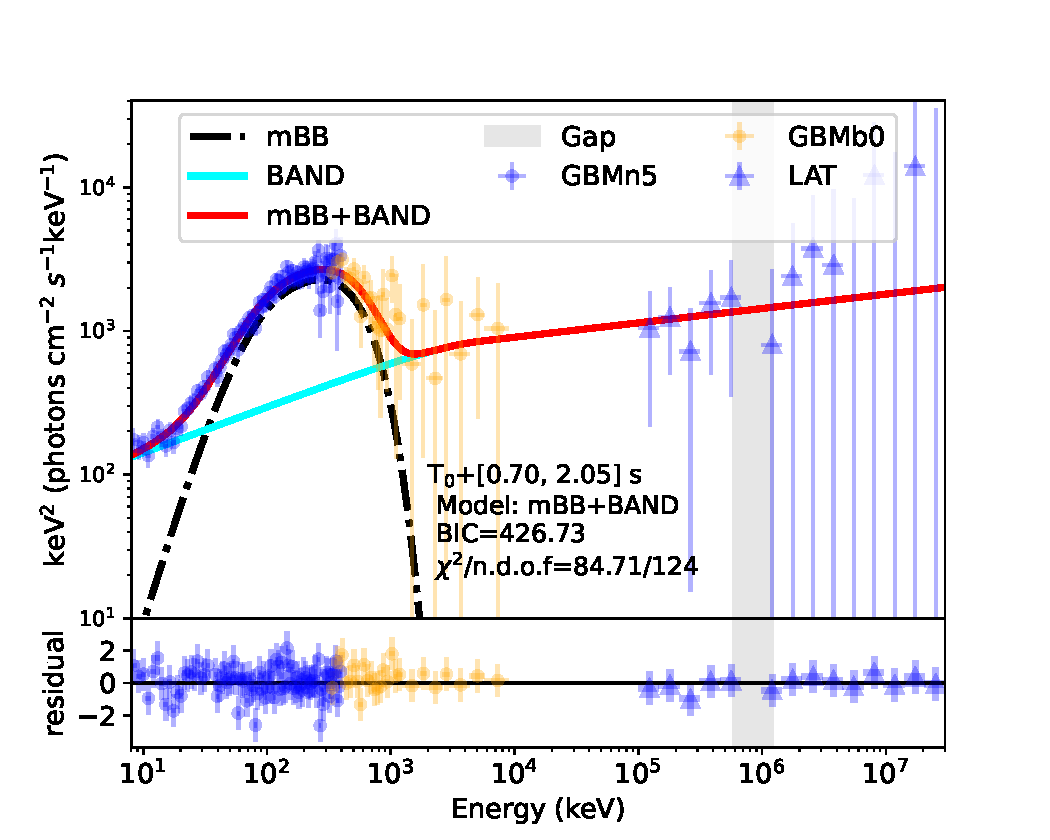
\includegraphics[width=.5\textwidth]{Fv_mBBBAND0_GRB210704A.pdf}\put(-90,140){(d) }
\\
\caption{Modeling results with BAND, BB+BAND, mBB+PL and mBB+BAND (modeling without zero-count bins in the gap).\label{fig:spectra2}}
\end{center}
\end{figure*}

%\fi
%\clearpage
%\clearpage
%TC:endignore
\bibliography{LIV}
\bibliographystyle{aasjournal}

\end{document}

% End of file `sample631.tex'.
